\documentclass[12pt,letterpaper]{article}
\usepackage{amsmath}
\usepackage{amsfonts}
\usepackage[figurewithin=section,tablewithin=section]{caption}
\usepackage[usenames,dvipsnames]{color}
\usepackage{graphicx}
\usepackage{longtable}
\usepackage{rotating}
\usepackage{booktabs}
\usepackage[bibencoding=utf8, citestyle=authoryear,bibstyle=authoryear,maxbibnames=99]{biblatex}
%\addbibresource{~/Projects/MyBibtex.bib}

\bibliography{/home/jsibert/Projects/MyBibtex.bib,/home/jsibert/MendeleyBibTex/library.bib}


\usepackage[pdftex,bookmarks=false]{hyperref}
\hypersetup{pdfauthor={John Sibert}
            pdfsubject={variable transmission and mortality rate estimates}
            pdftitle={Simple SIR Statistical Model}
            pdfkeywords={COVID-19, SIR Model, random effects, TMB}
            }%

\newcommand\doublespacing{\baselineskip=1.6\normalbaselineskip}
\newcommand\singlespacing{\baselineskip=1.0\normalbaselineskip}
\newcommand\help[1]{\color{Magenta}{\it #1 }\normalcolor}
\newcommand\EG{e.g.\ }
\newcommand\perda{$\rm{da}^{-1}$}
\newcommand\SSm{{\tt simpleSIR4}}

\title{Estimating short term trends in transmission and mortality rates
during the Covid 19 Epidemic}

\author{
John Sibert\thanks{sibert@hawaii.edu; johnrsibert@gmail.com}\\
Joint Institute of Marine and Atmospheric Research\\
University of Hawai`i at M\={a}noa\\
Honolulu, HI  96822 U.S.A.\\[0.125in]
\date{\today}
}

\pagestyle{headings}
\markright{John Sibert \hfil Simple SIR COVID-19 \hfil \today}

\begin{document}

\maketitle

\doublespacing

\begin{abstract}

\centerline{\help{Write me}}

{\parindent=0truein

TO DO:

Rationalize examples

Implement alternate ordinate scale

Make linear plots of I and D?
}
\end{abstract}

\section*{Introduction}

The sudden advent of the COVID-19 pandemic provoked many political
jurisdictions to advise people to ``shelter in place'' and to practice
``social distancing''. If this advice has been effective, it should be
possible to detect the effects of the advice by comparing changes in
numbers of infected people and perhaps changes in transmission rates
over time and
between areas. The SIR models of epidemic spread divide the affected
population into three compartments: 
Susceptible, Infected and Recovered.
SIR models are
usually expressed as coupled ordinary differential equations,
\begin{eqnarray}
\label{eqn:SIR}
\frac{dS}{dt} &=& -\beta\frac{IS}{N} - \mu S\\
\frac{dI}{dt} &=& \hphantom{-}\beta\frac{IS}{N} - \mu I -\gamma I\\
\frac{dR}{dt} &=&  -\mu R +\gamma I\\
N &=& S + I + R
\end{eqnarray}
where $N$ is the population size, $\beta$ is the instantaneous
transmission rate ($[t^{-1}]$), $\mu$ is the instantaneous mortality rate
($[t^{-1}]$),  and $\gamma$ is the instantaneous recovery rate
($[t^{-1}]$).  

%https://en.wikipedia.org/wiki/Compartmental_models_in_epidemiology
\cite{Chen2020,Roques2020}

Unfortunately, few data sets include data for each of
these compartments. 
The New York Times' ``historical'' 
data\footnote{\label{ff:nyt}\url{https://github.com/nytimes/covid-19-data/}}
is an easily accessible source of data. These
data comprise daily totals of ``cases'' and ``deaths'' for each county
in the United States. I assume that the data included as ``cases'' are
a reasonable approximations of the Infected compartment ($I$) in a SIR model. 
There are simply no credible data of comparable scope on either the Susceptible or
the Recovered compartments.

\section*{Model Structure}
I make some simplifying assumptions in the face of incomplete data: 
(1) The entire population is susceptible so that $S/N = 1$. 
(2) Over the short term, the size of the
Susceptible compartment does not change, 
$\frac{dS}{dt} = 0 = \frac{dN}{dt}$,
eliminating the Susceptible compartment.
(3) People who recover from a COVID-19 infection return to the Susceptible
compartment, eliminating the Recovered compartment. 
With these assumptions, and with the addition of a ``deaths''
compartment, the simplified SIR model is
\begin{eqnarray}
\label{eqn:sSIR}
\frac{dI}{dt} &=&  \beta I - \mu I -\gamma I\\
\frac{dD}{dt} &=& \mu I
\end{eqnarray}
and has state variables that might be matched to available observations.

The data available during the initial stages of the COVID-19 pandemic
contain measurement errors of various types.
Definitions and methods of detecting and reporting the numbers of
infected persons vary between political jurisdictions (or
``geographies'' in the parlance of the New York Times) and may also
change with time.
Comparable uncertainties also occur in reporting of deaths caused
by COVID-19 infection.
There is additional variability in the biosocial
processes that mediate disease transmission.

State-space models separate variability in the biosocial
processes in the system (transition model)
from errors in observing features of interest
in the system (observation model).
(See \cite{Harvey1990}).

The general form of a state-space process or transition model is
\begin{equation}
\alpha_t=T(\alpha_{t-1}) + \eta_t
\end{equation}
where $\alpha_t$ is the state at time $t$ and 
the function $T$ embodies the dynamics mediating the
development of the state at time $t$ from the state at the previous
time with random process error, $\eta_t$.

The transition model for the simplified SIR model is constructed from finite difference
approximations of equation (\ref{eqn:sSIR}) with associated log-normal
random errors.
\begin{eqnarray}
\label{eqn:sSIRfdI}
I_t &=& I_{t-\Delta t}\big(1+\Delta t(\beta_{t-\Delta t} - \mu_{t-\Delta t}
- \gamma_{t-\Delta t})\big)e^{\eta_t}\\
\label{eqn:sSIRfdD}
D_t &=& \big(D_{t-\Delta t} + \Delta t \mu_{t-\Delta t}I_{t-\Delta
t}\big)e^{\eta_t}
\end{eqnarray}
where $\eta$ is a normal random deviate, $\eta\sim
N(0,\sigma_\eta)$, representing temporal variability in the biosocial
factors that mediate the spread of the pandemic. 
The recovery rate, $\gamma_{t-\Delta t}$, in equation
(\ref{eqn:sSIRfdI}) is computed algebraically as
\begin{equation}
\gamma_{t-\Delta t} = \beta_{t-\Delta t} - \mu_{t-\Delta t} +
(1-\frac{I_t}{I_{t-\Delta t}})
\end{equation}
I have no particular
justification, beyond the parsimony principle, for the assumption that
the variance, $\sigma_\eta$, of the processes for $I$ and $D$, should be the
same.

One approach to modeling time-dependent rates of transmission and
mortality, $\beta$ and $\mu$, is to treat them as random effects
(\cite{Skaug2006}). Random effects are appropriate if repeating a time
series of observations would not yield the same outcome as the initial
observations. Random effects are also appropriate when observing
the same process in two different areas. I model the  $\beta$ and
$\mu$ time series as log-normal random walks. I assume that
\begin{eqnarray}
\log\beta_t &=& \log\beta_{t-\Delta t}+\varepsilon;\quad \varepsilon\sim 
N(0,\sigma_\beta)\\
\log\mu_t &=& \log\mu_{t-\Delta t}+\varrho;\quad \varrho\sim
N(0,\sigma_\mu)
\end{eqnarray}

The general form of the state-space observation model is
\begin{equation}
x_t = O(\alpha_t) + \varphi_t
\end{equation}
where the function $O$ describes the measurement process with
error $\varepsilon$ in observing the state $\alpha$.

I applied separate observation error models for cases and
deaths. The observation model for cases is a simple log-normal error
\begin{equation}
\label{eqn:logNlike}
\log\varphi_t = \bigg(\log\frac{1}{\sqrt{2\pi\sigma^2_I}} -\Bigl(\frac{\log
I_t-\log\widehat{I}_t}{\sigma_I}\Bigr)^2\bigg)\\
\end{equation}
where $I$ is the observed number of cases and $\widehat{I}$ is the
number of cases predicted by equation~\ref{eqn:sSIRfdI}.


Not all those afflicted by COVID-19 have died; there are far fewer
deaths than infections. In addition,
the observed time series for both $I$ and $D$ begins at the first recorded
case. The first recorded death occurs several days or weeks after the
first recorded case. 
Therefor the deaths time-series inevitably contains a
substantial number of recorded zeros. 
The observation model for deaths accommodates observed zeroes by
assuming to be ``zero-inflated'' log normal likelihood given by
\begin{equation}
\label{eqn:ZIlogNlike}
  \log \varepsilon_t = \left\{
    \begin{array}{r@{\;:\quad}l}
       D_t > 0 &
(1-p_0)\cdot\bigg(\log\frac{1}{\sqrt{2\pi\sigma^2_D}}
          -\Bigl(\frac{\log D_t-\log\widehat{D}_t}{\sigma_D}\Bigr)^2\bigg)\\
       D_t = 0 & p_0 \cdot\log \frac{1}{\sqrt{2\pi\sigma^2_D}}\\
    \end{array}
  \right.
\end{equation}
where $D$ is the observed number of deaths,
$\widehat{D}$ is the number of deaths predicted by
equation~\ref{eqn:sSIRfdD}, 
and $p_0$ is the proportion of observed deaths equal to zero.


Model parameters are estimated by
maximizing the joint likelihood of the process errors, observation
errors, and random effects.
\begin{equation}
\label{eqn:likelihood}
L(\theta,\alpha,x)=
\prod^m_{t=2}\big[\phi\big(\alpha_t-T(\alpha_{t-1}), \Sigma_\eta\big)\big]\cdot
\prod^m_{t=1}\big[\phi\big(x_t-O(\alpha_t),
\Sigma_\varepsilon\big)\big]
\end{equation}
where $m$ is the number of days elapsed since the first recorded case,
$x_t$ is the vector of daily observations of cases and deaths,
$\alpha_t$ is the vector of the daily calculations of the state
variables and random effects,
and $\theta$ 
is a vector of model parameters (Table~\ref{tab:allvars1}).
The R package TMB (\cite{TMB0000} package was used to 
estimate the parameters of the model. 
The R and supporting C++ files are available on 
github.\footnote{\SSm~at \url{https://github.com/johnrsibert/SIR-Models}}

\begin{table}
\caption{List of model variables for the simple SIR model, \SSm.
There are two state variables computed from the of estimated
parameters and random effects.
There are two random effects and five estimated variance parameters.
All models variables are represented in the TMB C++ module as their
natural logarithms.
}
\label{tab:allvars1}
\begin{center}
\begin{tabular}{ll}
\hline
Variable & Definition\\
\hline
\hline
       & {\it State variables:}\\
$I$      & Number of infected individuals\\
$D$      & Number of deaths\\
       & {\it Random effects:}\\
$\beta_t$ & Transmission rate; log-normal random walk\\
$\mu_t$   & Mortality rate; log-normal random walk\\
       & {\it Estimated parameters:}\\
$\sigma_I$ & Infectious compartment estimation standard deviation\\
$\sigma_D$ & Deaths compartment estimation standard deviation\\
$\sigma_\eta$ & Standard deviation of transmission and deaths process errors\\
$\sigma_\beta$ & Standard deviation of transmission rate random walk\\
$\sigma_\mu$ & Standard deviation of mortality rate random walk\\
\hline
\end{tabular}
\end{center}
\end{table}

%\clearpage
\section*{Results}

\begin{figure}
\begin{center}
\includegraphics[width=1.00\textwidth]{../Graphics/counties_per_capita.png}
\end{center}
\caption{\label{fig:percap}
Trends in number of cases per 1000 people in the 30 most populous US
counties.
The vertical gray bar mark the March 19, 2020 California shelter in place order.
}
\end{figure}

%All data are derived from the New York times github 
%site\footnote{See note \ref{ff:nyt}.}.
% {\url{https://github.com/nytimes/covid-19-data/}}. 

Trends in the per-capita number of cases in the thirty largest counties in the
United States are shown in Figure~(\ref{fig:percap}).
These trajectories fall into two more or less distinct groups: those
that are concave downward, \EG Nassau Co. NY (NaNY), and those that are
concave upward, \EG Miami-Dade Co. FL (MDFL).


\begin{figure}
{\scriptsize
\begin{center}
\includegraphics[width=0.80\textwidth]{../Graphics/NassauNY_prevalence.png}
 
\vspace{0.25truein}

\includegraphics[width=0.80\textwidth]{../Graphics/Miami-DadeFL_prevalence.png}
\end{center}
}
\caption{\label{fig:prev}
Prevalence trajectories for six US counties.
Blue bars indicate daily increases increases in cases and deaths;
dark blue lines indicate 11 day moving averages of daily increases
(labeled ``11da''); 
pale blue lines indicate cumulative numbers (labeled $\Sigma C$ and
$\Sigma D$); 
vertical gray bar marks the March 19, 2020 California shelter in place order.
\help{remove annotations.}
}
\end{figure}

Prevalence histories for six counties are shown in
Figure~\ref{fig:prev} where the 11-day moving averages of the daily
increases in cases and deaths indicate general trends.
All of the histories show extreme day to day variability.
Variability is most notable in the deaths
time series, particularly for smaller counties.

This model, \SSm , estimates two random effects and five
parameters, Table~\ref{tab:allvars1}.
In principle, all random effects and parameters are estimated
simultaneously.
Performance of the estimation model depends on
model configuration. When all parameters and random effects are
estimated, the numerical algorithm fails converge for some counties,
see Table~\ref{tab:uncons}. Column `C' in the table
indicates the convergence status of attempts to fit several county
trajectories using the relatively robust Nelder-Mead function
minimization algorithm (\cite{Baudin2010}).
Convergence is signaled by values of C equal to
zero.\footnote{According to the R documentation for the {\tt optim}
function: An integer code. ‘0’
indicates successful completion.  Possible error codes are
          ‘1’ indicates that the iteration limit ‘maxit’ had been
              reached.
          ‘10’ indicates degeneracy of the Nelder-Mead simplex.
}


Diagnostic plots for the unconstrained model are shown in figures~\ref{fig:ests1U}
and~ \ref{fig:ests2U} for convex downward and convex upward trajectories
respectively. \label{pp:diagexpl}
Diagnostics are plotted on logarithmic scales to illustrate the
lognormal likelihood functions used in the observation model,
equations (\ref{eqn:logNlike}) and (\ref{eqn:ZIlogNlike}), and to
illustrate trends in estimated rates that are near zero.
The blue `+' symbols represent the observed cases ($I$) and deaths ($D$).
The red lines overlaying the symbols are model predictions ($\widehat{I}$)
and ($\widehat{D}$) of cases and deaths. 
$\sigma_I$ and $\sigma_D$ are the estimated standard deviations of
cases and deaths in the observation model.
The shaded areas bounded by red outlines are 
$\pm 2$ estimated standard deviations around the estimated trends.
The model reproduces the observed numbers of cases and deaths almost
exactly with extremely low estimates of $\sigma_I$ and $\sigma_D$.

The solid blue lines in the $\beta$ and $\mu$ diagnostic plots are the estimated
transmission and death rate random effects.
The shaded areas bounded by blue outlines are
estimated random effects $\pm 2$ standard deviations of the generating
random walks.
\help{Omit these? 
The red lines labeled $\tilde{\beta}$ and $\tilde{\mu}$ are the
medians of the two random effects.}
The extreme variability in the data is reflected in the extreme
variability of the estimated trends in transmission and mortality rates.

The \SSm\ model can be configured with $\sigma_I$ and $\sigma_D$ fixed at
constant values. The results are shown in Table~\ref{tab:cons}. 
The algorithm converges to a solution in all cases, and converges
rapidly using gradient methods.
Constrained model diagnostic plots
values are shown in figures \ref{fig:ests1} and
\ref{fig:ests2} for convex downward and convex upward trajectories
respectively.
Estimated cases and deaths agree well with observation throughout the
time series.

Figure~\ref{fig:xrates} compares estimated transmission rate among
counties.
Transmission rates increased rapidly at the beginning of the pandemic
exceeding  $-1$ in early March, an instantaneous transmission rate equivalent to a 
doubling time of less than one day.
Beginning in April, transmission rates fell substantially, and doubling times
increased to longer than 3 weeks in some counties.
Counties with estimated $\ln~ \beta \le 5$ at the of May
correspond roughly to those counties with concave downward prevalence
trajectories.


\begin{figure}
\begin{center}
\includegraphics[width=1.00\textwidth]{../Graphics/constrainID/logbeta_summary.png}\\
\end{center}
\caption{\label{fig:xrates}
Estimated natural logarithms of the transmission rate for several US counties using the
constrained \SSm\ model.
Values of $\ln \beta > -2$ indicate doubling times ($t_2$) less than 5 days;
$\ln~ \beta < -4$ indicate doubling times greater than 35 days.
$t_2 = \frac{\ln 2}{\exp(\ln \beta)}$
}
\end{figure}

\begin{figure}
\begin{center}
\includegraphics[width=1.00\textwidth]{../Graphics/constrainID/logmu_summary.png}\\
\end{center}
\caption{\label{fig:drates}
Estimated natural logarithms of the mortality rate for several US counties using the
constrained \SSm\ model.
exp(-8) = 0.00033
\help{Remove ToNY, Tompkins Co NY}
}
\end{figure}

\section*{Discussion}

Nonlinear statistical models with multiple estimated parameters rely
on numerical methods to estimate parameters by searching for minima
(hopefully finding only one) in the negative of the likelihood
function. The parameter values at the minima are considered to be
maximum likelihood estimators. Failure to find well defined minima is
usually a cause for concern. The minimization algorithms applied to
unconstrained \SSm\ do not reliably converge to a solution. The
standard deviations in the observation model are components of the
likelihood, and the algorithm therefore pushes these parameters toward zero.
Since the estimated parameters in \SSm\ are represented as logarithms,
they cannot take values $\le$ zero. Restricting the values of
$\sigma_I$ and $\sigma_D$ to small, but non-zero, constants allows the
algorithm to estimate the other parameters.

The trends in estimated transmission rate Figure~\ref{fig:xrates} seem
reasonable. The extremely high transmission rates in March agree well
with doubling times reported in newspaper articles at the time.
The steady decline of transmission rates after shelter-in-place advice is 
also consistent with casual observation.
The incubation time of the COVID-19 virus is usually assumed to be
about 14 days.
The trends in Figure~\ref{fig:xrates} in conjunction with the
empirical prevalence trends suggest that sustainable containment of
the pandemic does not occur unless the instantaneous transmission rate
is forced below $0.018 da^{-1}$, that is, unless the doubling time is greater
than 35 days, approximately twice the incubation period.

\help{
Upward bump in transmission rates consistent with observed increases
in cases in July.


Omit:
Whether the available data are sufficiently informative to enable
estimation of the model parameters is a critical aspect of the
evaluation of any statistical model.
The speed at which the COVID-19 pandemic spread during the first
quarter of
2020 means that the length of the time series doubled during
the development of this model. The capability of the
model improve conveniently during the model development period,
but whether the improvement is
attributable to changes in model structure or to the increase in the
length of the time series is unclear. This ambiguity influenced the
development of the model.}

\cite{Sibert2017,Nielsen2014b}


\clearpage

\begin{sidewaystable}
\caption{\label{tab:uncons}
Model results. Estimating $\beta$ and $\mu$ trends as random effects
with computed $\gamma$
Data updated 2020-07-22 from
https://github.com/nytimes/covid-19-data.git.
}
\centering
{\small
%%%%%%%%%%%%%% :r ../fits/fit_table.tex


\begin{tabular}{lrrrrrrrrrrrr}
\hline
 County            &   $n$ &   $p_0$ &   $f$ &   $C$ &   $\sigma_\eta$ &   $\sigma_\beta$ &   $\sigma_\mu$ &   $\sigma_I$ &   $\sigma_D$ &   $\tilde\gamma$ &   $\tilde{\beta}$ &   $\tilde{\mu}$ \\
\hline
 Nassau, NY        &   138 &  0.0863 &  -945 &     1 &           0.193 &            0.557 &          3.37  &     9.77e-05 &     2.42e-05 &        -9.45e-09 &           0.0035  &        0.000171 \\
 New York City, NY &   142 &  0.0909 &  -834 &     0 &           0.196 &            1.06  &          1.02  &     0.000522 &     0.000493 &        -2.73e-08 &           0.00583 &        0.000278 \\
 Cook, IL          &   179 &  0.294  &  -978 &     1 &           0.136 &            3.09  &          0.854 &     9.24e-08 &     0.000126 &        -2.24e-07 &           0.00926 &        0.000299 \\
 Honolulu, HI      &   137 &  0.181  & -1470 &    10 &           0.149 &            2.94  &         14.6   &     0.000346 &     2.68e-07 &        -5.51e-08 &           0.0108  &        2.24e-12 \\
 Philadelphia, PA  &   133 &  0.112  &  -608 &     1 &           0.167 &            1.02  &          1.98  &     0.00279  &     0.00452  &        -3.1e-08  &           0.0117  &        0.0003   \\
 Bexar, TX         &   160 &  0.242  &  -650 &    10 &           0.123 &            2.58  &          7.21  &     0.00236  &     1.76e-05 &        -7.18e-08 &           0.028   &        4.64e-07 \\
 Tarrant, TX       &   133 &  0.0746 &  -570 &     1 &           0.146 &            1.23  &          1.36  &     0.0102   &     0.00327  &        -3.78e-08 &           0.0305  &        0.000279 \\
 Palm Beach, FL    &   131 &  0.0758 &  -428 &     1 &           0.143 &            0.339 &          1.36  &     0.0873   &     0.00614  &        -1.17e-08 &           0.0308  &        0.000658 \\
 Harris, TX        &   138 &  0.101  &  -380 &     1 &           0.117 &            0.266 &          0.894 &     0.167    &     0.0226   &        -2.15e-08 &           0.0308  &        0.000278 \\
 Miami-Dade, FL    &   132 &  0.12   &  -618 &     1 &           0.159 &            0.606 &          0.995 &     0.000848 &     0.00583  &        -9.54e-09 &           0.0328  &        0.000493 \\
 Hillsborough, FL  &   142 &  0.175  &  -722 &     1 &           0.119 &            3.69  &         11.7   &     1.78e-07 &     4.86e-08 &        -7.24e-08 &           0.0355  &        4.64e-05 \\
 Travis, TX        &   130 &  0.107  &  -350 &     0 &           0.122 &            0.244 &          1.71  &     0.188    &     0.00726  &        -1.6e-08  &           0.0358  &        0.000243 \\
 Maricopa, AZ      &   177 &  0.303  &  -885 &     1 &           0.118 &            2.13  &          2.33  &     3.62e-07 &     0.000867 &        -4.2e-07  &           0.0367  &        0.000321 \\
 Dallas, TX        &   133 &  0.0672 &  -452 &     1 &           0.136 &            0.3   &          1.19  &     0.0798   &     0.00953  &        -1.04e-08 &           0.0371  &        0.000405 \\
 Broward, FL       &   137 &  0.0797 &  -511 &     0 &           0.136 &            0.231 &          1.66  &     0.0799   &     0.00289  &        -2.03e-08 &           0.038   &        0.000275 \\
\hline
 Median            &   137 &  0.107  &  -618 &     1 &           0.136 &            1.02  &          1.66  &     0.00236  &     0.00289  &        -2.73e-08 &           0.0308  &        0.000278 \\
\hline
\end{tabular}


%%%%%%%%%%%%%%%%
}\end{sidewaystable}


\begin{figure}
{\scriptsize
\begin{center}
\begin{tabular}{ll}
\multicolumn{1}{c}{New York City}&\multicolumn{1}{c}{Cook Co. IL}\\
\includegraphics[width=0.50\textwidth]{../Graphics/unconstrained/New_York_CityNY_TMB_estimates.png}&
\includegraphics[width=0.50\textwidth]{../Graphics/unconstrained/CookIL_TMB_estimates.png}\\
\\
\multicolumn{1}{c}{Nassau Co. NY}&\multicolumn{1}{c}{Philadelphia Co.  PA}\\
\includegraphics[width=0.50\textwidth]{../Graphics/unconstrained/NassauNY_TMB_estimates.png}&
\includegraphics[width=0.50\textwidth]{../Graphics/unconstrained/PhiladelphiaPA_TMB_estimates.png}\\
\end{tabular}
\end{center}
}
\caption{\label{fig:ests1U}
Unconstrained model diagnostics for concave downward counties.
See page \pageref{pp:diagexpl}for explanation of plots.
}
\end{figure}

\begin{figure}
{\scriptsize
\begin{center}
\begin{tabular}{ll}
\multicolumn{1}{c}{Miami-Dade Co. FL}&\multicolumn{1}{c}{Maricopa Co. AZ}\\
\includegraphics[width=0.50\textwidth]{../Graphics/unconstrained/Miami-DadeFL_TMB_estimates.png}&
\includegraphics[width=0.50\textwidth]{../Graphics/unconstrained/MaricopaAZ_TMB_estimates.png}\\
\\
\multicolumn{1}{c}{Palm Beach Co. FL}&\multicolumn{1}{c}{Travis Co. TX}\\
\includegraphics[width=0.50\textwidth]{../Graphics/unconstrained/Palm_BeachFL_TMB_estimates.png}&
\includegraphics[width=0.50\textwidth]{../Graphics/unconstrained/TravisTX_TMB_estimates.png}\\
\end{tabular}
\end{center}
}
\caption{\label{fig:ests2U}
Unconstrained model diagnostics for concave upward counties.
}
\end{figure}


\begin{sidewaystable}
\caption{\label{tab:cons}
Model results. Estimating $\beta$ and $\mu$ trends as random effects with computed $\gamma$
and constraints on  $\sigma_I$ and $\sigma_D$. 
Data updated 2020-07-22 from
https://github.com/nytimes/covid-19-data.git.
}
\centering
{\small
%%%%%%%%%%%%%% :r ../fits/fit_table.tex


\begin{tabular}{lrrrrrrrrrrrr}
\hline
 County            &   $n$ &   $p_0$ &    $f$ &   $C$ &   $\sigma_\eta$ &   $\sigma_\beta$ &   $\sigma_\mu$ &   $\sigma_I$ &   $\sigma_D$ &   $\tilde\gamma$ &   $\tilde{\beta}$ &   $\tilde{\mu}$ \\
\hline
 Nassau, NY        & 143   &  0.0833 & -170   &     0 &         0.139   &           0.23   &         0.26   &        0.405 &        0.223 &       -1.4e-08   &           0.00468 &       0.000341  \\
 New York City, NY & 147   &  0.0878 & -137   &     0 &         0.158   &           0.211  &         0.202  &        0.405 &        0.223 &       -2.22e-08  &           0.00712 &       0.000592  \\
 Philadelphia, PA  & 138   &  0.108  & -187   &     0 &         0.123   &           0.179  &         0.17   &        0.405 &        0.223 &       -2.36e-08  &           0.0127  &       0.0011    \\
 Honolulu, HI      & 142   &  0.175  & -329   &     0 &         0.068   &           0.193  &         0.242  &        0.405 &        0.223 &       -4.87e-08  &           0.0197  &       0.000274  \\
 Alameda, CA       & 147   &  0.149  & -312   &     0 &         0.079   &           0.118  &         0.14   &        0.405 &        0.223 &       -3.54e-08  &           0.0239  &       0.000581  \\
 Tarrant, TX       & 138   &  0.0719 & -254   &     0 &         0.0948  &           0.123  &         0.264  &        0.405 &        0.223 &       -3.12e-08  &           0.0301  &       0.000557  \\
 Palm Beach, FL    & 136   &  0.073  & -218   &     0 &         0.111   &           0.161  &         0.146  &        0.405 &        0.223 &       -1.77e-08  &           0.0303  &       0.0011    \\
 Cook, IL          & 184   &  0.286  & -284   &     0 &         0.098   &           0.197  &         0.145  &        0.405 &        0.223 &       -2.19e-07  &           0.0305  &       0.00186   \\
 Dallas, TX        & 138   &  0.0647 & -229   &     0 &         0.106   &           0.148  &         0.162  &        0.405 &        0.223 &       -1.74e-08  &           0.0309  &       0.000615  \\
 Harris, TX        & 143   &  0.0972 & -243   &     0 &         0.0987  &           0.149  &         0.159  &        0.405 &        0.223 &       -2.93e-08  &           0.0319  &       0.000414  \\
 Travis, TX        & 135   &  0.103  & -229   &     0 &         0.098   &           0.16   &         0.141  &        0.405 &        0.223 &       -2.02e-08  &           0.035   &       0.000492  \\
 Miami-Dade, FL    & 137   &  0.116  & -170   &     0 &         0.132   &           0.197  &         0.147  &        0.405 &        0.223 &       -1.25e-08  &           0.0356  &       0.000683  \\
 Broward, FL       & 142   &  0.0769 & -242   &     0 &         0.105   &           0.166  &         0.128  &        0.405 &        0.223 &       -2.26e-08  &           0.0375  &       0.000619  \\
 Hillsborough, FL  & 147   &  0.169  & -303   &     0 &         0.0781  &           0.159  &         0.126  &        0.405 &        0.223 &       -6.51e-08  &           0.0424  &       0.000886  \\
 Maricopa, AZ      & 182   &  0.295  & -314   &     0 &         0.085   &           0.202  &         0.0985 &        0.405 &        0.223 &       -3.74e-07  &           0.0426  &       0.00198   \\
 Bexar, TX         & 165   &  0.235  & -351   &     0 &         0.0663  &           0.139  &         0.204  &        0.405 &        0.223 &       -8.07e-08  &           0.0508  &       0.000552  \\
\hline
 Median            & 142.5 &  0.1055 & -242.5 &     0 &         0.09835 &           0.1635 &         0.153  &        0.405 &        0.223 &       -2.645e-08 &           0.0307  &       0.0006035 \\
\hline
\end{tabular}


%%%%%%%%%%%%%%%%
}\end{sidewaystable}

\begin{figure}
{\scriptsize
\begin{center}
\begin{tabular}{ll}
\multicolumn{1}{c}{New York City}&\multicolumn{1}{c}{Cook Co. IL}\\
\includegraphics[width=0.50\textwidth]{../Graphics/constrainID/New_York_CityNY_TMB_estimates.png}&
\includegraphics[width=0.50\textwidth]{../Graphics/constrainID/CookIL_TMB_estimates.png}\\
\\
\multicolumn{1}{c}{Nassau Co. NY}&\multicolumn{1}{c}{Philadelphia Co.  PA}\\
\includegraphics[width=0.50\textwidth]{../Graphics/constrainID/NassauNY_TMB_estimates.png}&
\includegraphics[width=0.50\textwidth]{../Graphics/constrainID/PhiladelphiaPA_TMB_estimates.png}\\
\end{tabular}
\end{center}
}
\caption{\label{fig:ests1}
Model diagnostics for concave downward counties.
}
\end{figure}

\begin{figure}
{\scriptsize
\begin{center}
\begin{tabular}{ll}
\multicolumn{1}{c}{Miami-Dade Co. FL}&\multicolumn{1}{c}{Maricopa Co. AZ}\\
\includegraphics[width=0.50\textwidth]{../Graphics/constrainID/Miami-DadeFL_TMB_estimates.png}&
\includegraphics[width=0.50\textwidth]{../Graphics/constrainID/MaricopaAZ_TMB_estimates.png}\\
\\
\multicolumn{1}{c}{Palm Beach Co. FL}&\multicolumn{1}{c}{Travis Co. TX}\\
\includegraphics[width=0.50\textwidth]{../Graphics/constrainID/Palm_BeachFL_TMB_estimates.png}&
\includegraphics[width=0.50\textwidth]{../Graphics/constrainID/TravisTX_TMB_estimates.png}\\
\end{tabular}
\end{center}
}
\caption{\label{fig:ests2}
Model diagnostics for concave upward counties.
}
\end{figure}

\clearpage
\printbibliography[title=References]

\end{document}


%An integer code. 0 indicates successful completion (which is always the case for "SANN" and "Brent"). Possible error codes are
%
%1
%
    %indicates that the iteration limit maxit had been reached.
%10
%
    %indicates degeneracy of the Nelder--Mead simplex.
%


\begin{figure}
{\scriptsize
\begin{center}
\begin{tabular}{ll}
\multicolumn{1}{c}{New York City}&\multicolumn{1}{c}{Cook Co. IL}\\
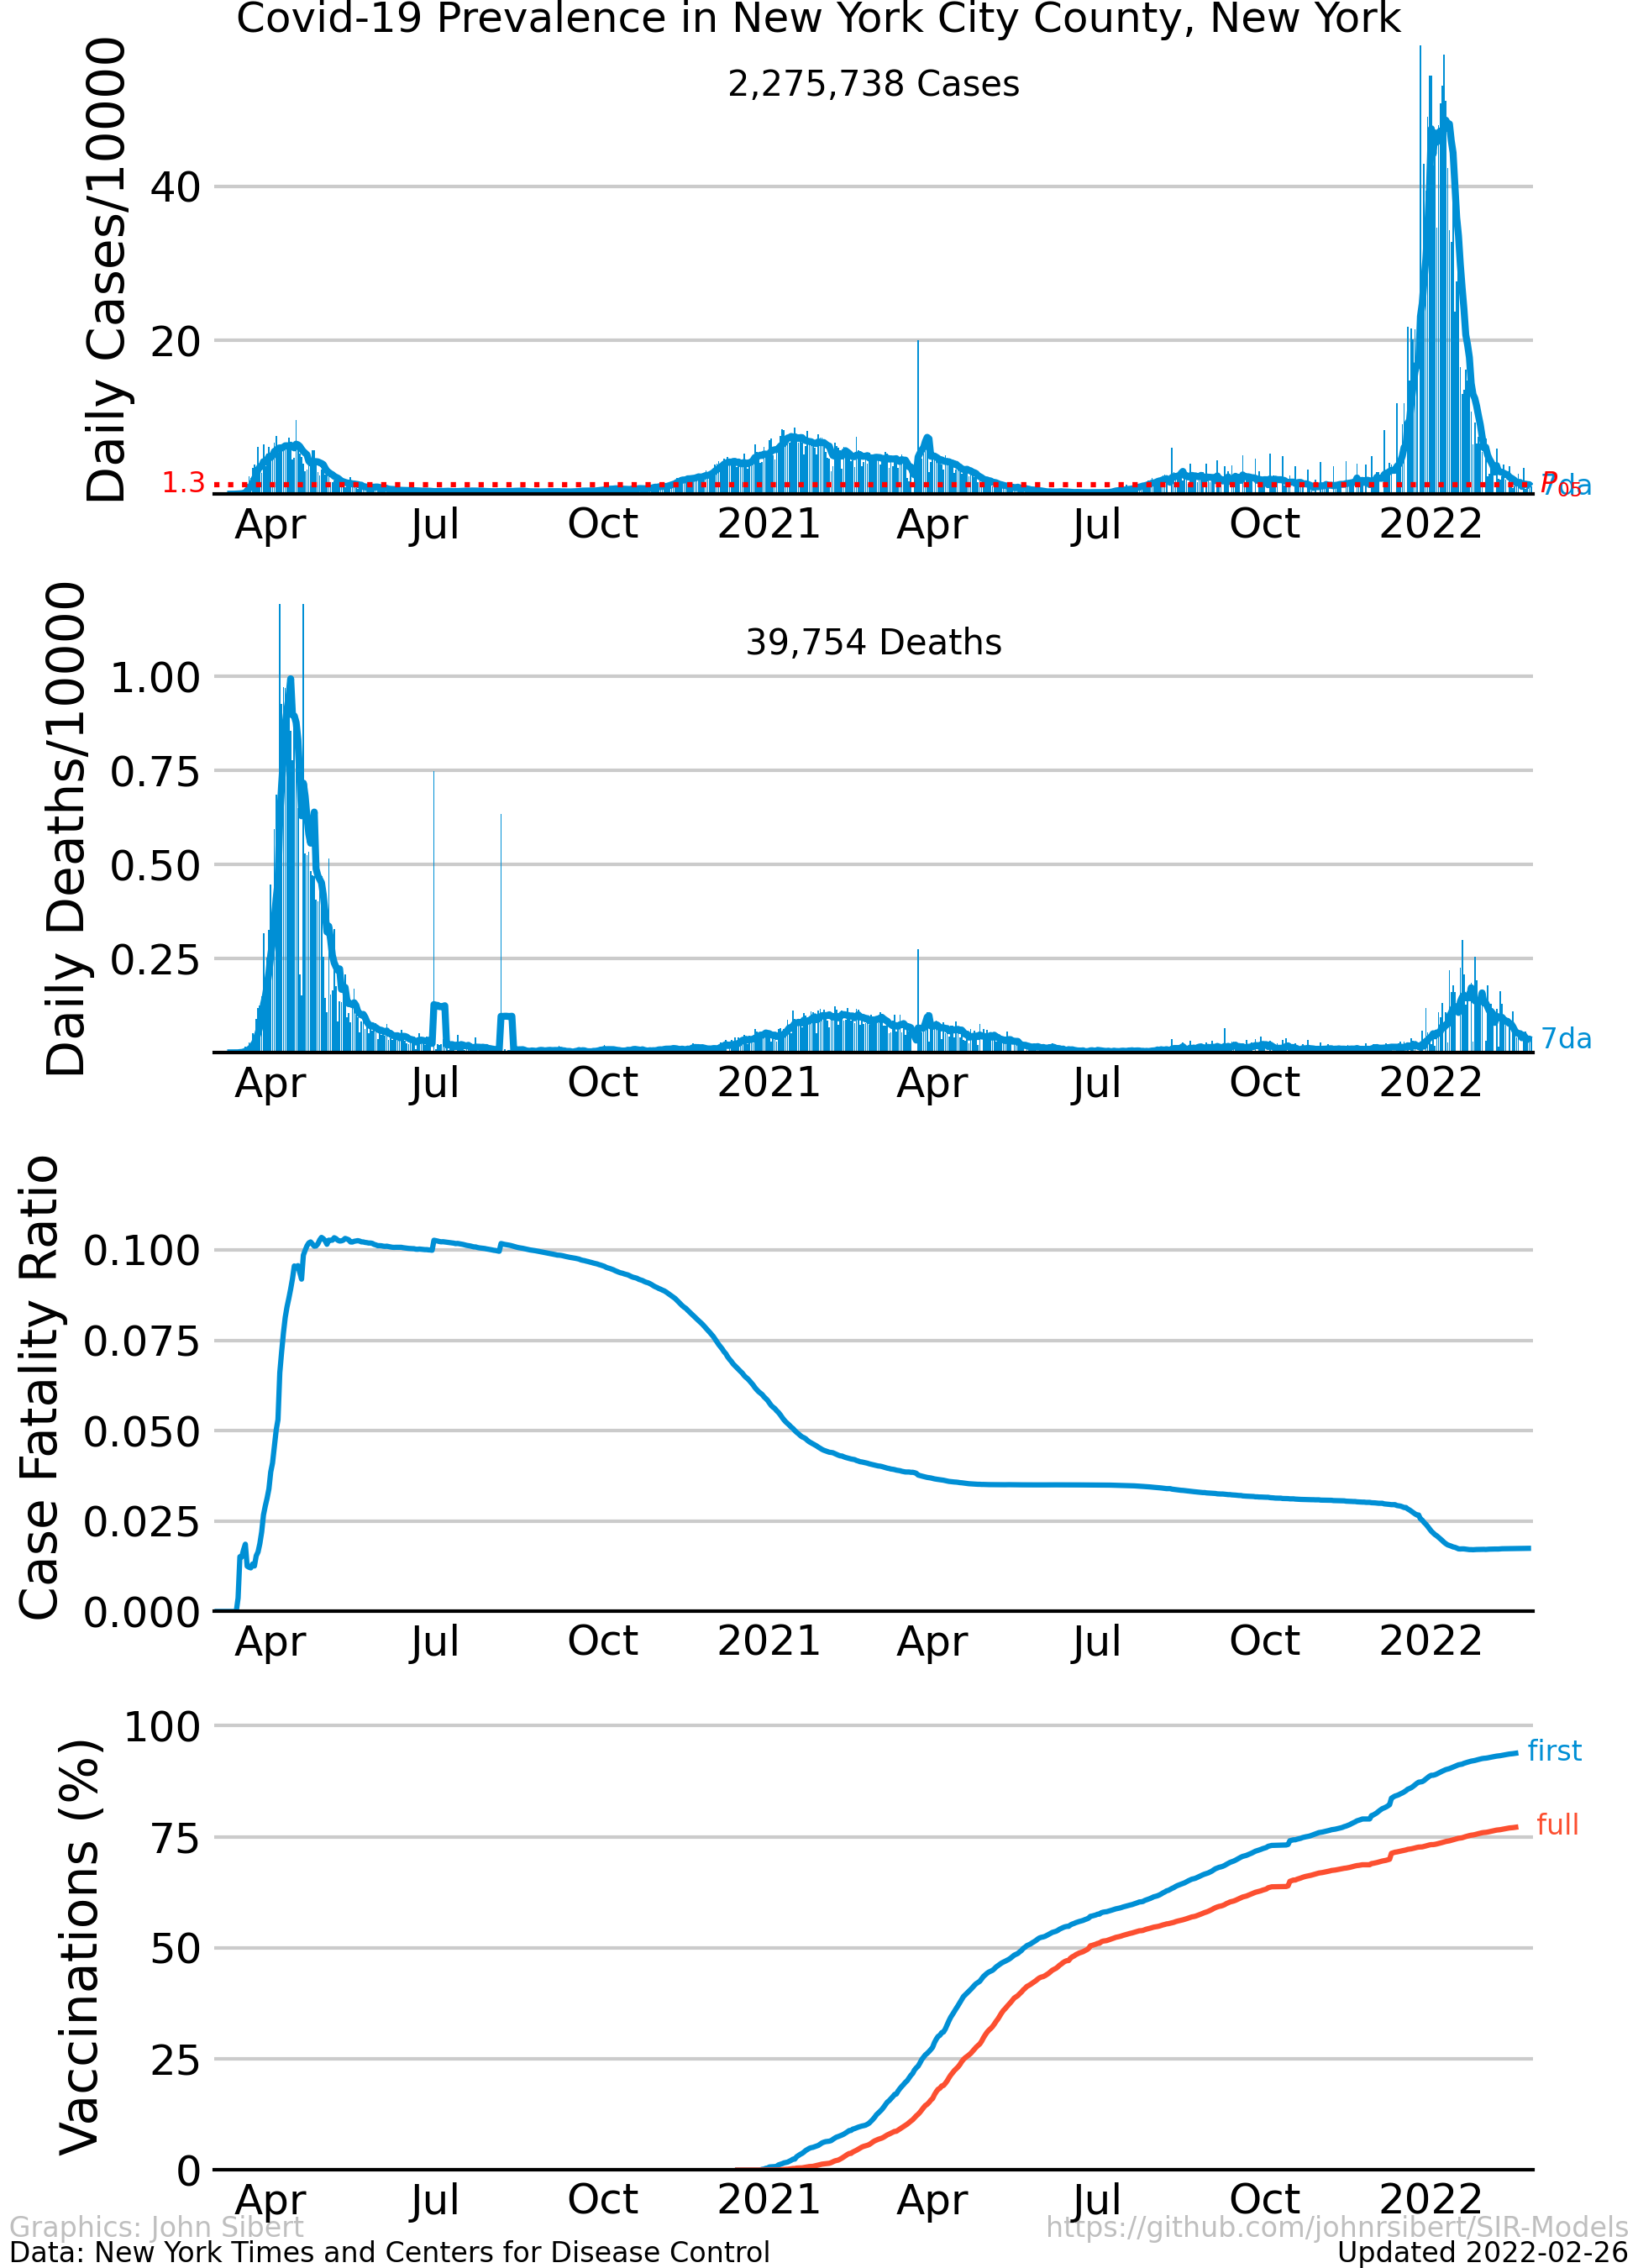
\includegraphics[width=0.50\textwidth]{../Graphics/New_York_CityNY_prevalence.png}&
\includegraphics[width=0.50\textwidth]{../Graphics/CookIL_prevalence.png}\\
\\
\multicolumn{1}{c}{Miami-Dade Co. FL}&\multicolumn{1}{c}{Maricopa Co. AZ}\\
\includegraphics[width=0.50\textwidth]{../Graphics/Miami-DadeFL_prevalence.png}&
\includegraphics[width=0.50\textwidth]{../Graphics/MaricopaAZ_prevalence.png}\\
\\
\multicolumn{1}{c}{Broward Co. FL}&\multicolumn{1}{c}{Travis Co. TX}\\
\includegraphics[width=0.50\textwidth]{../Graphics/BrowardFL_prevalence.png}&
\includegraphics[width=0.50\textwidth]{../Graphics/TravisTX_prevalence.png}\\
\end{tabular}
\end{center}
}
\caption{\label{fig:prev}
Prevalence trajectories for six US counties.
Blue bars indicate daily increases increases in cases and deaths;
dark blue lines indicate 11 day moving averages of daily increases
(labeled ``11da''); 
pale blue lines indicate cumulative numbers (labeled $\Sigma C$ and
$\Sigma D$); 
vertical gray bar marks the March 19, 2020 California shelter in place order.
\help{remove annotations.}
}
\end{figure}

